\chapter{Speech Emotion Recognition Using Acoustic Features}
\chaptermark{SER using acoustic feature}

% \section{Introduction}
The purpose of this chapter is three-fold: (1) to investigate the effective
region of analysis for acoustic feature extraction, whether frame-based region
(local features) or utterance-based region (global features); (2) to evaluate
which action is the best with regard of silence region in dimensional speech
emotion recognition (SER); and (3) to
evaluate which aggregation method performs better for dimensional SER: acoustic
input aggregation or outputs aggregation, like majority voting method. 

\section{Which region of analysis to extract acoustic features in SER}
\sectionmark{Region of Analysis}
\subsection{SER using low-level acoustic features}
% introduce frame-based processing
SER in conventional ways are performed by extracting acoustic features on
frame-based processing and then applied these features to a classifier. Let
$y(n)$, with $ n = 1, 2, 3, \ldots , L$, denotes acoustic signal with length
$L$.  In frame-based processing, this $y(n)$ signal is divided into frames by
fixed length. A typical length for a single frame is 16-25 milliseconds (ms)
with 10 ms to 15 ms hop length (stride). For 25 ms frame length and 10 ms hop
length, which is equal to 60\% overlap (15 ms), a window is applied to this
frame to make the short-time signal behave as quasistationary signal -- near
stationary signal. In their original length, an acoustic signal vary with the
time: non-stationary property.  Windowing processes acoustic signal in
short-term interval to remove this property. Figure \ref{fig:frame-processing}
shows the windowing process; short-term windowed signals look more stationary
than the original signal.

% # Windowing: why 25 ms, add figure, why overlapping

Windowing multiplies spectrum of input signal with window signal $w(n)$.  A
typical window function for acoustic signal is Hann and Hamming windows (named
after Julius von Hann and Richard W. Hamming).  The others are rectangular,
Bartlet, Kaiser, and Blackman.  The choice of window function is based
on two aspects: width of main lobe and additional lobes. Hann and Hamming
windows only differ in weighting factors with similar concept: cosine-sum
windows

\begin{equation}
  w[n] = A + B \cos \biggl(\frac {2\pi n}{M}\biggl), ~~~~~n = -M/2, \ldots, M/2,
\end{equation}

\noindent where $A$ is $0.5$ for Hann and $0.54$ for Hamming. $B$ is $0.5$ for
Hann and $0.46$ for Hamming. Both window functions are widely used in speech
processing due to good trade-off between time and frequency resolution (effect
of side lobes). Figure \ref{fig:window_hann} shows Hann window and its spectrum,
while Figure \ref{fig:windowing_demo} shows an example of Hamming window applied
to sinusoid signal and its result.

\begin{figure}[htbp]
  \centering
  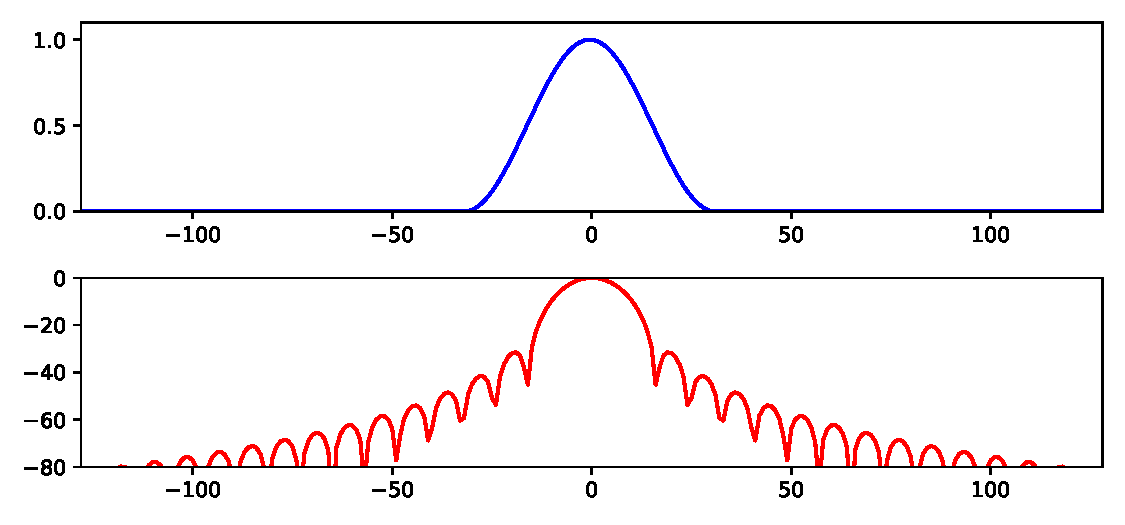
\includegraphics[width=\textwidth]{../fig/window_hann.pdf}
  \caption{Hann window and its spectrum}
  \label{fig:window_hann}
\end{figure}

\begin{figure}[htbp]
  \centering
  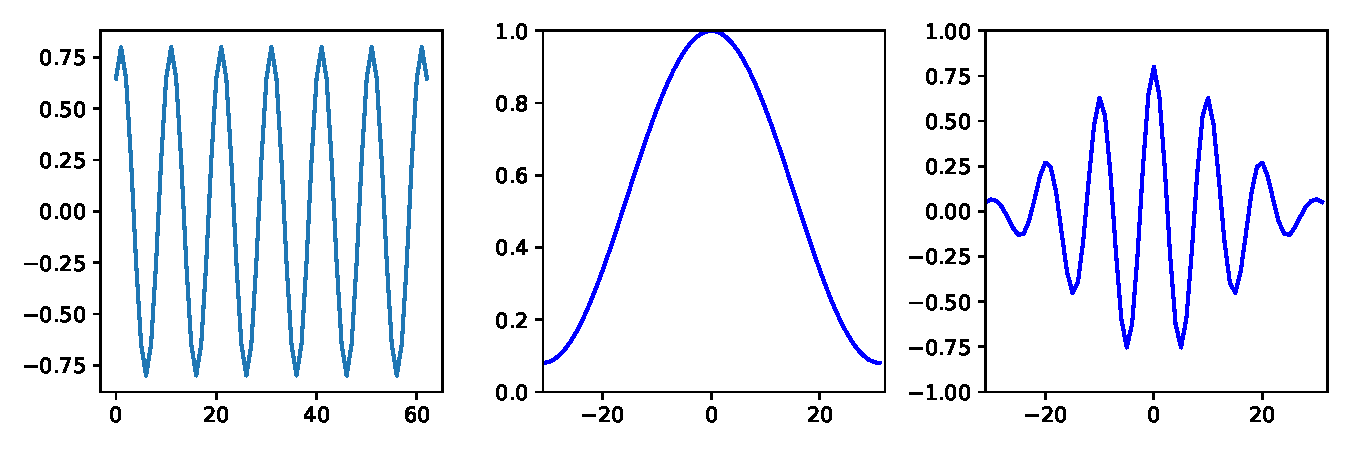
\includegraphics[width=\textwidth]{../fig/windowing_demo.pdf}
  \caption{An example of Hamming window (middle) applied to sinusoid signal (left); the resulted windowed signal (right) is multiplication of both.}
  \label{fig:windowing_demo}

\end{figure}
The length of a window is usually equal to the length of frame: one window per
frame. If the length of a window is smaller than a frame, each frame will be
windowed with window length and padded with zeros to match length of frame. It
costs more computation. In speech emotion recognition, short window is used to
capture short dynamics context while longer window is used to capture mid and
longer dynamics. A common approach used short window to extract acoustic
features in short-term time while long-term dynamics are modeled by statistical 
functions. Figure \ref{fig:frame-processing} shows frame-based processing of an
acoustic signal (speech) which windows short-term signals using Hamming window.

\begin{figure}[htbp]
  \centering
  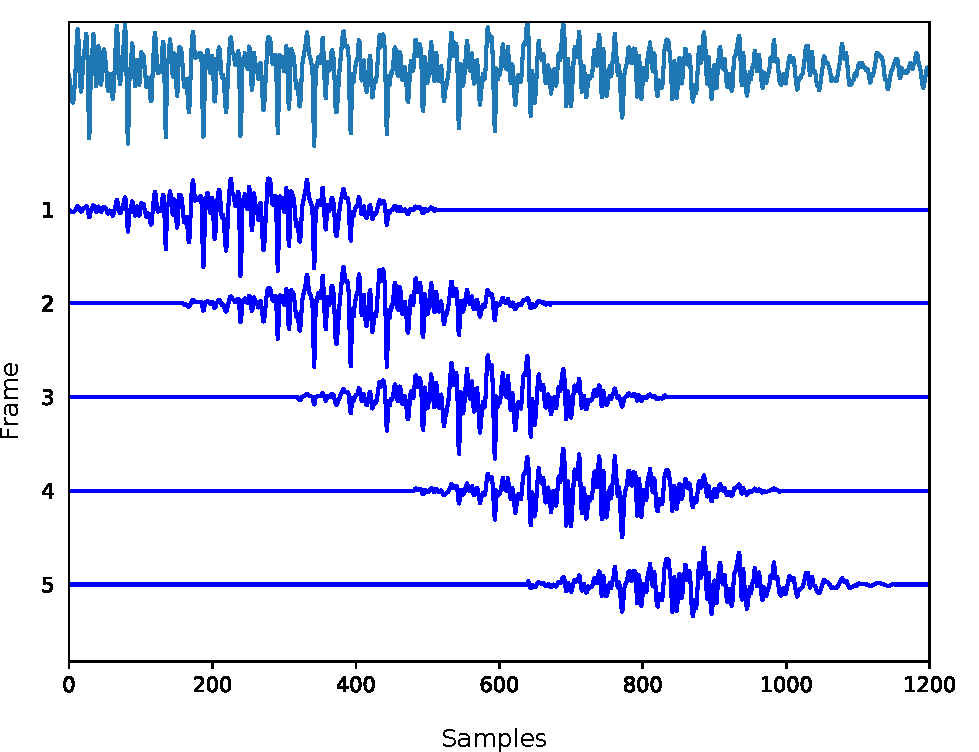
\includegraphics[width=\textwidth]{../fig/framing.pdf}  
  \caption{Frame-based processing for extracting low-level descriptors of an acoustic signal; the signal is an excerpt of IEMOCAP utterance with 400 samples frame length and 160 samples hop length; sampling frequency is 16 kHz.}
  \label{fig:frame-processing}
\end{figure}

% # LLD, MFCC, Why
The acoustic features extracted on each frame are known as local features or
low-level descriptor (LLD) \cite{Herrera1999}. The most common LLD for speech
processing is mel-frequency cepstral coefficients (MFCC). MFCC captures
different aspects of the spectral shape of a speech. The following steps
compute MFCC in sequences. First, FFT/DFT transformed time domain signal into
frequency domain signal (spectra). Second, mel frequency warping function
convert spectra in linear scale into mel scale. Although several functions have
been proposed, a common approach keeps linear scale for acoustic frequencies
below 1 kHz and converts to logarithmic scale for acoustic frequencies above 1
kHz. This conversion imitates human perceptual system. Third, convert a power
spectrogram (amplitude squared) to decibel (dB) units ($\log$). Finally, DCT
computes MFCC as amplitude cepstra.

% number of mfcc coefficients; number of frame; shape of MFCC
One of the important parameters in MFCC is the number of coefficients. A number
of 13 to 40 coefficients are common for speech processing. For each frame 13
MFCCs are extracted. If there are 40 frames in an utterance, the dimension of
MFCC features will be (40, 13). Obviously, the number of frames corresponds to
the number of samples divided by hop length (in samples).  If an utterance
comprises 1 second (s) with 16000 Hz sampling rate, the number of samples is
16000. Using 25 ms (400 samples) window/frame length and 10 ms (160 samples)
hop length, the number of frames is $16000/160$, i.e., 100 frames. Figure
\ref{fig:mfcc-mel} top shows an MFCC spectrogram of an IEMOCAP utterance with 13
coefficients.

% mel-spectrogram and log mel-spectrogram
Recently, researchers found that mel-spectrogram, also called as (mel) filter
bank and mel frequency spectral coefficients (MFSC), yields a better
performance for deep learning-based automatic speech recognition (ASR) (e.g.,
\cite{Mohamed2014}). Given that deep learning system is less susceptible with
high correlated input, the DCT step in previous MFCC calculation is not
necessary since it is linear transformation.  DCT discards some information in
speech signals which are highly non-linear \cite{fayek2016}. Furthermore, a log
version (in decibel unit) of mel-spectrogram, i.e., log mel-spectrogram, is
preferable one since deep learning learns better in this unit. The conversion
from mel-spectrogram to log mel-spectrogram is given by

\begin{equation}
  S_{dB} = 10 \log \biggl( \frac {S}{ref}\biggr),
  \label{eq:log-mel}
\end{equation}
\noindent where $S$ is the input power spectrogram and $ref$ is reference
power. A value of $1.0$ is a common $ref$ value for 32-bit floating-point
wav data (`float32').

% show and interpret figure
Figure \ref{fig:mfcc-mel} shows visualization of MFCC, mel-spectrogram and log
mel-spectrogram. From this figure, it is clear that log mel-spectrogram is more
informative than mel-spectrogram and MFCC. This visualization may support the
previous argument that log mel-spectrogram may works better in DNN-based
speech emotion recognition.

\begin{figure}[htbp]
  \centering
  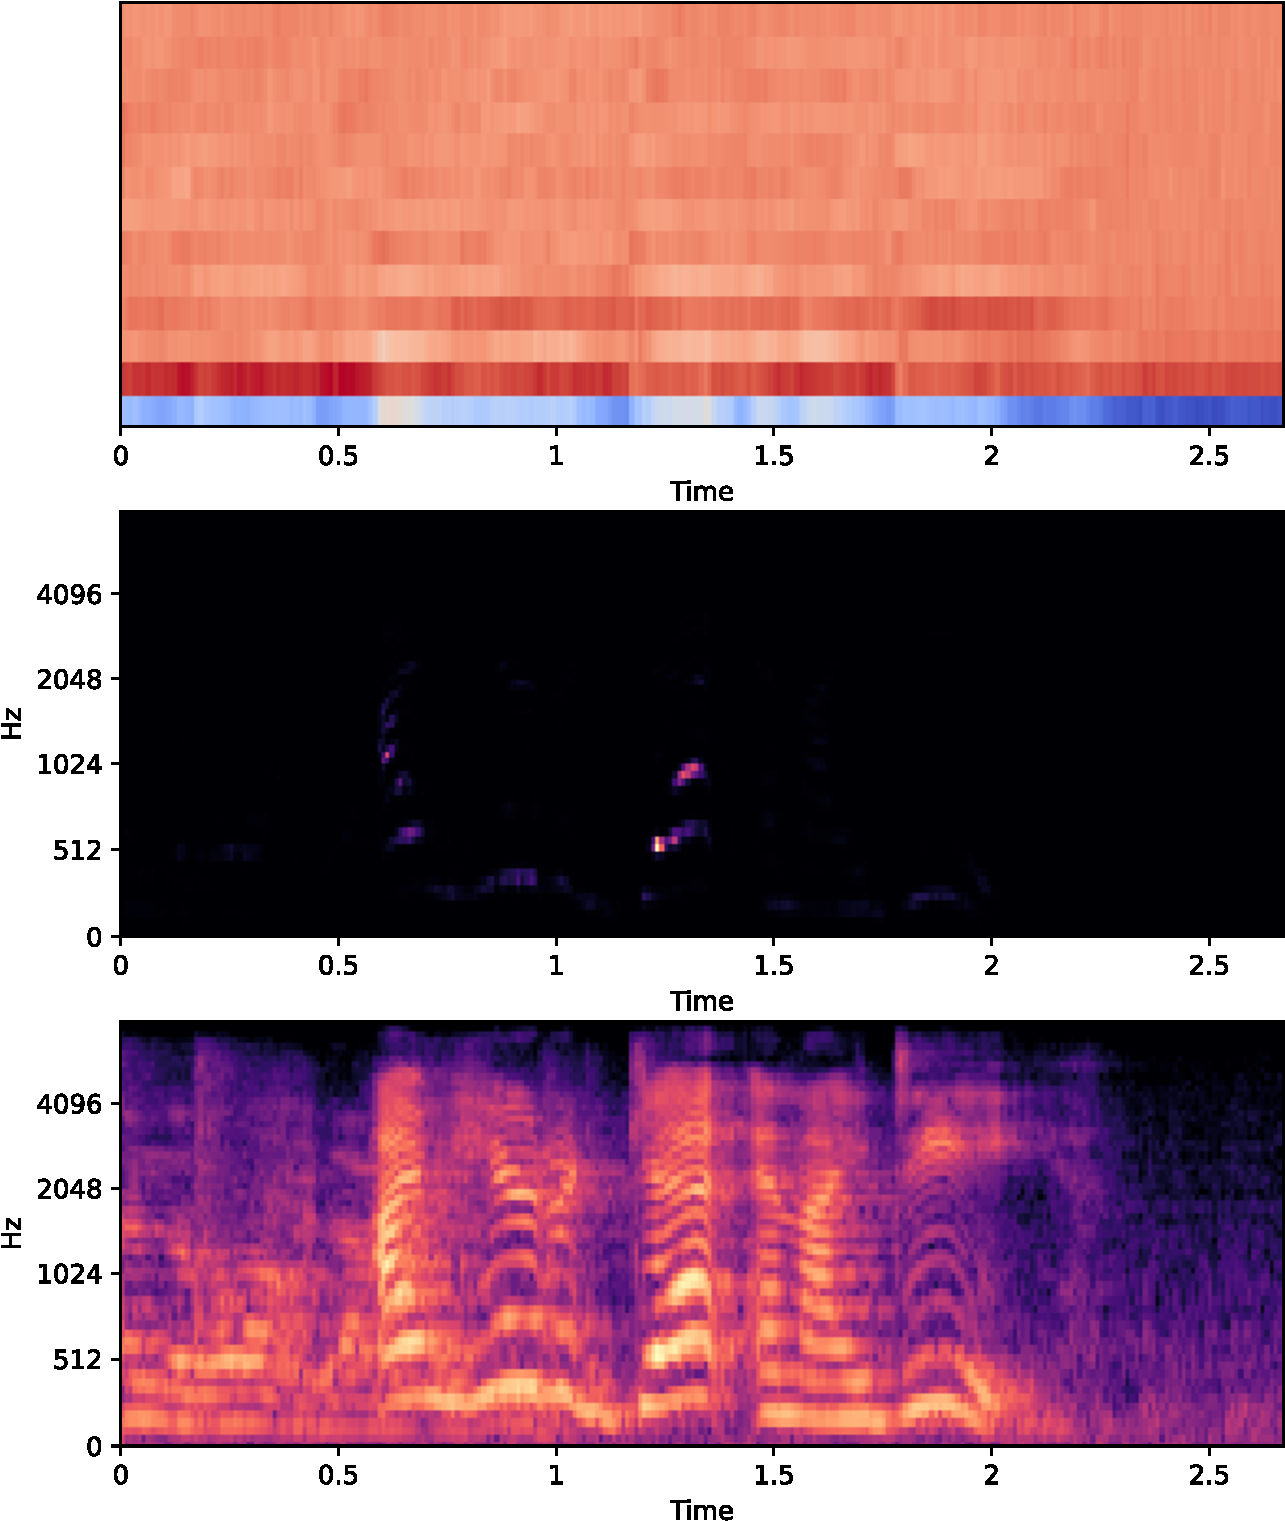
\includegraphics[width=.7\textwidth]{../fig/mfcc-mel-crop.pdf}
  \caption{Visualization of MFCC features with 13 coefficients (top), 
  mel-spectrogram middle, and log mel-spectrogram with 64 mels.}
  \label{fig:mfcc-mel}
\end{figure}

Apart from the use of one type acoustic features for speech processing, some
researchers have proposed a set of acoustic features for speech emotion
recognition. Eyben et al. \cite{Eyben} proposed Geneva minimalistic parameter
set (GeMAPS) as standard acoustic features for affective voice research. The
proposed acoustic features are based on: (1) physiological changes in voice
production, (2) proven significance in previous studies, and (3) theoretical
significance. The proposed acoustic features comprises 23 LLDs as shown in
Table \ref{tab:gemaps_paa}. This acoustic feature set is extracted on
frame-processing basis with 25 ms frame length and 10 ms hop length.

% pyAudioanalysis
Giannakopulos \cite{Giannakopoulos2015} proposed pyAudioanalysis as an open
source Python library for audio signal analysis. The library supports a wide
range of audio analysis procedures such as feature extraction, classification,
supervised and unsupervised segmentation, and visualization. Different from
GeMAPS feature set, pyAudioanalysis targets a wide range of voice application
like audio event detection, speech emotion recognition, music segmentation, and
health application. The short-term feature set, which is extracted on
frame-processing basis, consists of 34 LLDs. These LLDs are shown in Table 
\ref{tab:gemaps_paa}.

\begin{table}[htpb]
\caption{Acoustic feature sets: GeMAPS \cite{Eyben} and pyAudioAnalysis
\cite{Giannakopoulos2015}. The numbers in parentheses indicate the total
numbers of features (LLDs).}
\label{tab:gemaps_paa}
  \begin{center}
  \begin{tabular}{p{7.5cm} | p{7cm}}
  \hline 
  \hspace{2.5cm}GeMAPs (23) & \hspace{1.5cm}pyAudioAnalysis (34) \\
  \hline \hline
intensity, alpha ratio, Hammarberg index, spectral slope 0-500 Hz, spectral
slope 500-1500 Hz, spectral flux, 4 MFCCs, $f_o$, jitter, shimmer,
harmonics-to-noise ratio (HNR), harmonic difference H1-H2, harmonic difference
H1-A3, F1, F1 bandwidth, F1 amplitude, F2, F2 amplitude, F3, and F3 amplitude.
& zero crossing rate, energy, entropy of energy, spectral centroid, spectral
spread, spectral entropy, spectral flux, spectral roll-off, 13 MFCCs, 12 chroma
vectors, chroma deviation.\\
  \hline 
  \end{tabular}
\end{center}
 \end{table}

% Result
As additional features sets, a temporal difference on pyAudioAnalysis were
computed in first order, referred as \emph{deltas}. The addition of first order
regression coefficients shows better a performance than original LLDs (MFCC and
MFSC) in ASR. In dimensional SER, these temporal difference may show the
dynamics between frames. Together with previous four feature sets, these LDDs
are compared to evaluate the effectiveness of frame-based LLDs in dimensional
SER. 

% interpret tabel
Table \ref{tab:iemocap-lld} shows performance of dimensional SER from IEMOCAP
dataset in CCC score. 

\begin{table}
    \caption{Results of frame-based LLDs for dimensional SER in IEMOCAP dataset}
    \begin{center}
    \begin{tabular}{l | c | c c c c}
      \hline 
      Feature & Dim & Val & Aro & Dom & Mean \\
      \hline \hline
      MFCC	    & (3414, 40)	  &0.148	  & 0.488	  & 0.419	  & 0.352 \\
      Log Mel	  & (3414, 128)   &0.103    & 0.543   & 0.438   & 0.362 \\
      GeMAPS	  & (3409, 23)	  &0.164	  & 0.527	  & 0.454	  & 0.382 \\
      pAA	      & (3412, 34)	  &0.130	  & 0.513	  & 0.419	  & 0.354 \\
      pAA+D	    & (3412, 68)	  &0.145	  & 0.526	  & 0.439	  & 0.370 \\
      \hline
    \end{tabular}
    \label{tab:iemocap-lld}
  \end{center}
\end{table}



% Summary LLD and Problem with frame-based processing: high-dimensions, needs
% zero padding

\subsection{SER using high-level acoustic features}
% GeMAPS
In the previous subsection, it is shown that frame-based acoustic features work
with limited performance. In this subsection, the effectiveness of two
statistical functions is shown. Two high-level acoustic features, i.e., mean
values and standard deviations from LLDs are evaluated from the previous five
acoustic feature sets. 

% describe mean
The first high-level acoustic features used for this dimensional SER task is
mean values. The idea of using this mean values is to capture the common
information across all frames. This mean values can be formulated as

\begin{equation}
  \mu_F = \frac{1}{\mathcal{K}}\sum _{i=1}^n F_i  
\end{equation}

\noindent where $\mathcal{K}$ is the number of frames and $F$ is related
feature.  For instance, in pyAudioAnalysis, the first feature is zero crossing
rate (ZCR).  Mean values of ZCR feature is arithmetical mean of all ZCR values
in all frames within an utterance.  

% describe std
The second high-level acoustic features is standard deviation (std). This
statistical function shows the dispersion of feature values from its mean.
While mean is intended to capture the commonalities among features values in
all frames within an utterance, std is intended to capture the dynamics of
feature values in utterance. Accordingly, std is formulated as follows, 

\begin{equation}
  \sigma_F^2 = \frac{1}{\mathcal{K}}\sum _{i=1}^n (F_i - \mu_F)^2.
\end{equation}

% recap mean+std
Both mean and std (Mean+Std) are known as valuable functions in SER.
References \cite{Sebastian2019, Morales2016, Tomas2019} have used
Mean+Std for categorical SER. However, most references did not use only
Mean+Std, but other statistical functions like median, quartiles, minimum,
maximum and other features. It is interesting to experiment with Mean+Std only
for dimensional SER given the fact that both high-level features are two most
informative descriptors among others statistical functions. Beside reducing
size or dimension of features significantly, using Mean+Std consequently speed
up computation of SER with regard of their small input features.

Another advantage of using Mean+Std features is no need of zero padding.
Although zero padding is useful for FFT calculation (spectral smoothness), it
is unclear the effect of zero padding on LLDs for acoustic feature extraction.
Zero padded values may impact information represented by features when such
processing is performed, e.g., standardization or normalization. Hence,
acoustic features represented by Mean+Std features are more informative than
LLDs since it only contains information from speech. 

An illustration of Mean+Std extraction from LLDs is shown in Figure
\ref{fig:mean_std}. For instance, a MFCC features set from an utterance
consists of 3414 frames with 40 MFCC coefficients. For each mean and std
features, 40 values are calculated. Both mean and std are concatenated to form
Mean+Std features after transposing both statistical features.

\begin{figure}[htbp]
  \centering
  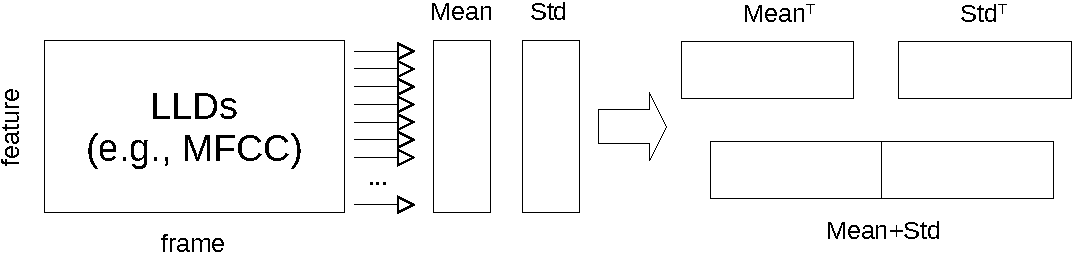
\includegraphics[width=0.9\textwidth]{../fig/mean_std-crop.pdf}
  \caption{Illustration of Mean+Std extraction from LLDs (e.g., MFCCs)}
  \label{fig:mean_std}
\end{figure}

% shows result

\begin{table}
    \caption{Results of frame-based LLDs for dimensional SER in IEMOCAP dataset}
    \begin{center}
    \begin{tabular}{l | c | c c c c}
      % \hline
      \hline
      Feature & Dim & Val & Aro & Dom & Mean \\
      \hline \hline
      MFCC      & 	40	& 0.155	& 0.580	  & 0.456 &	0.397 \\
      Log Mel	  &   128	& 0.151	& 0.549	  & 0.455 &	0.385 \\
      GeMAPS    & 	23	& 0.191	& 0.523	  & 0.452 &	0.389 \\
      pAA       & 	34	& 0.145	& 0.563	  & 0.445 &	0.384 \\
      pAA+D     & 	68	& 0.173	& 0.612	  & 0.455 &	0.413 \\
      \hline
      % \hline
    \end{tabular}
    \label{tab:iemocap-hsf}
  \end{center}
\end{table}

% show and discuss pAA+D obtain best performance
\subsection{Optimizing dimensional SER using different classifiers}
% \section{Evaluation Metric}
% \section{Experiment and Results on Region Analysis of Acoustic Features}
In the previous subsections, the study focuses in search of relevant acoustic 
features (regions) for feature extraction. As described in the previous
chapter, two important components of SER are features and classifiers. In this
subsection, a study to optimize dimensional SER using different classifiers is
presented. 

Long short-term memory (LSTM) networks is used to obtain the previous results
on both LLDs and Mean+Std features. The LSTM network consists of 3 layers with
256 units each. This configuration is based on \cite{Atmaja2020d}. Since the input is sequences of acoustic features, the use of
recurrent-based LSTM network is a straightforward approach. The use of LSTM as
classifier for SER have been found useful for both dimensional
\cite{Schmitt2018} and categorical task \cite{Atmaja2019}. While the previous
results used three layers with the same units, this optimization section varies
one to five layers with different number of units.

Apart from LSTM networks, convolutional neural networks (CNN) and multilayer
perceptrons (MLP) were accommodated. Both CNN and MLP use varying layers and
their corresponding units as shown in Table \ref{tab:layer}. CNN have found to
be useful for image-like input. Log mel-spectrogram is an example of this
input. MLP, one of the oldest neural network architecture, remains useful due
its simplicity to model complex internal representation of their environment
\cite{Hinton1989}. While the implementation of both LSTM and CNN were performed
by using Keras toolkit \cite{chollet2015keras}, the implementation of MLP was
performed using scikit-learn toolkit \cite{scikit-learn}.

\begin{table}
  \caption{Number of layer and corresponding units on each layer}
  \begin{center}
      \begin{tabular}{c  c}
          \hline
          \# layers   &   \# units \\
          \hline \hline
          1   &   (16) \\
          2   &   (32, 16) \\
          3   &   (64, 32, 16) \\
          4   &   (128, 64, 32, 16) \\
          5   &   (256, 128, 64, 32, 16) \\
          6   &   (512, 256, 128, 64, 32, 16) \\
          \hline
      \end{tabular}
      \label{tab:layer}
  \end{center}
\end{table} 

% interpret table
Table \ref{tab:iemocap-optim} shows result of optimizing dimensional SER using
different classifiers. As for the input, all networks take the previous
pyAudioAnalysis with deltas (pAA+D). Changing the number of layers and their
units changes their performances, as well as changing the classifiers. Using
CNN, and improvement from the previous LSTM result was obtained using a single
layer with 16 nodes. On using MLP, significant improvements were obtained; the
highest average CCC score was obtained using 5 layers. The average CCC score of
this architecture is 0.474.

\begin{table}
    \caption{Average CCC score on IEMOCAP dataset using different classifiers}
    \begin{center}
    \begin{tabular}{l | c c c c c c}
      \hline 
      Feature &   1lay	& 2lay	& 3lay	& 4lay	& 5lay	& 6lay  \\
      \hline \hline
      LSTM	& 0.389	& 0.403	& 0.385	& 0.401	& 0.395	& 0.399 \\
      CNN	  & 0.415	& 0.399	& 0.380	& 0.376	& 0.390	& 0.379 \\
      MLP	  & 0.450	& 0.469	& 0.448	& 0.462	& 0.472	& 0.452 \\
      \hline
    \end{tabular}
    \label{tab:iemocap-optim}
  \end{center}
\end{table}

% show and discuss why MLP obtain the best
To this end, several steps to observe which region of analysis to extract
acoustic features were performed. At first, the common LLDs, like MFCC
features, was evaluated. Later, the Mean+Std of these LLDs were used as input
features to the same classifier. The results show clearly that extracting
statistical functions over frame-based LLDs is better. Mean+Std with small size
($40$ vs. ($3414 \times 40$)) consistently performs better than LLDs. An
optimization using different classifiers shows improvements from the previous
LSTM networks with the same high-level acoustic features. 

\section{Effect of silent pause features in dimensional SER}
In the previous section, analysis of region for acoustic feature extraction was
investigated. This section investigates the second issue in dimensional SER
using acoustic features: which action is better to treat silence pause region
in dimensional SER. There are three actions can be taken regarding silent pause
in SER:
\begin{itemize}
  \item removing silence: extract acoustic features from speech-segment only,
\item keeping silence: extract acoustic features from whole utterance,
including speech and silence regions,
  \item utilizing silence: use silent pause regions as acoustic features.
\end{itemize}
The goal of this section is to examine which action from these three serves the
best for dimensional SER. The second action was already evaluated in the
previous results; therefore, only first and third actions will be explained and
evaluated in this section.

\subsection{Dimensional SER on silence-removed region}
% removing silence
Removing silence is a common practice in speech processing. ASR avoids
recording silence voice and only uses voiced speech to save power and
computational load. In automatic SER, the contribution of silence in speech is
not clear until now. Aguilar et al. \cite{Aguilar2020} evaluated both removing
and keeping silence for unimodal and multimodal categorical emotion
recognition. The result is different.  Keeping silences lead to better
performance in unimodal emotion recognition, while multimodal shows removing
silence is better than keeping silence. Atmaja and Akagi \cite{Atmaja2019}
shows that removing silence lead to higher accuracies score than using whole
speech in categorical speech emotion recognition. 

% calculating RMS
A naive way to calculate silence region within speech is by using root mean
square (RMS) energy. Given a threshold $\tau$, if the RMS energy of a speech
frame below this $\tau$ threshold, then that frame is categorized as a silence. 
The RMS energy is given by the following equation:
\begin{equation}
  x_{rms} = \sqrt{\dfrac{1}{n} (x_1^2 + x_2^2 + \ldots + x_n^2)}
\end{equation}
As shown in Figure \ref{fig:silence} (b), a threshold of $0.065$ is a reasonable
choice for given speech utterance (an excerpt from IEMOCAP dataset). However,
this RMS energy curve occasionally fall below the threshold for a moment and
these values are not counted as silence. A better way to detect silence is by
probability mapping, a conversion from raw RMS energy to a
likelihood/probability. The probability mapping is formulated as 
\begin{equation}
  P[S=1 | x_{rms}] = \frac{\exp(x_{rms} - \tau)}{1 + \exp(x_{rms} - \tau)}
\end{equation}
The result shown in Figure \ref{fig:silence} (c). The final part in the bottom
of the figure shows the result in binary value, an $S$ of 1 for silence and 0
for non silence.

\begin{figure}
  \centering
  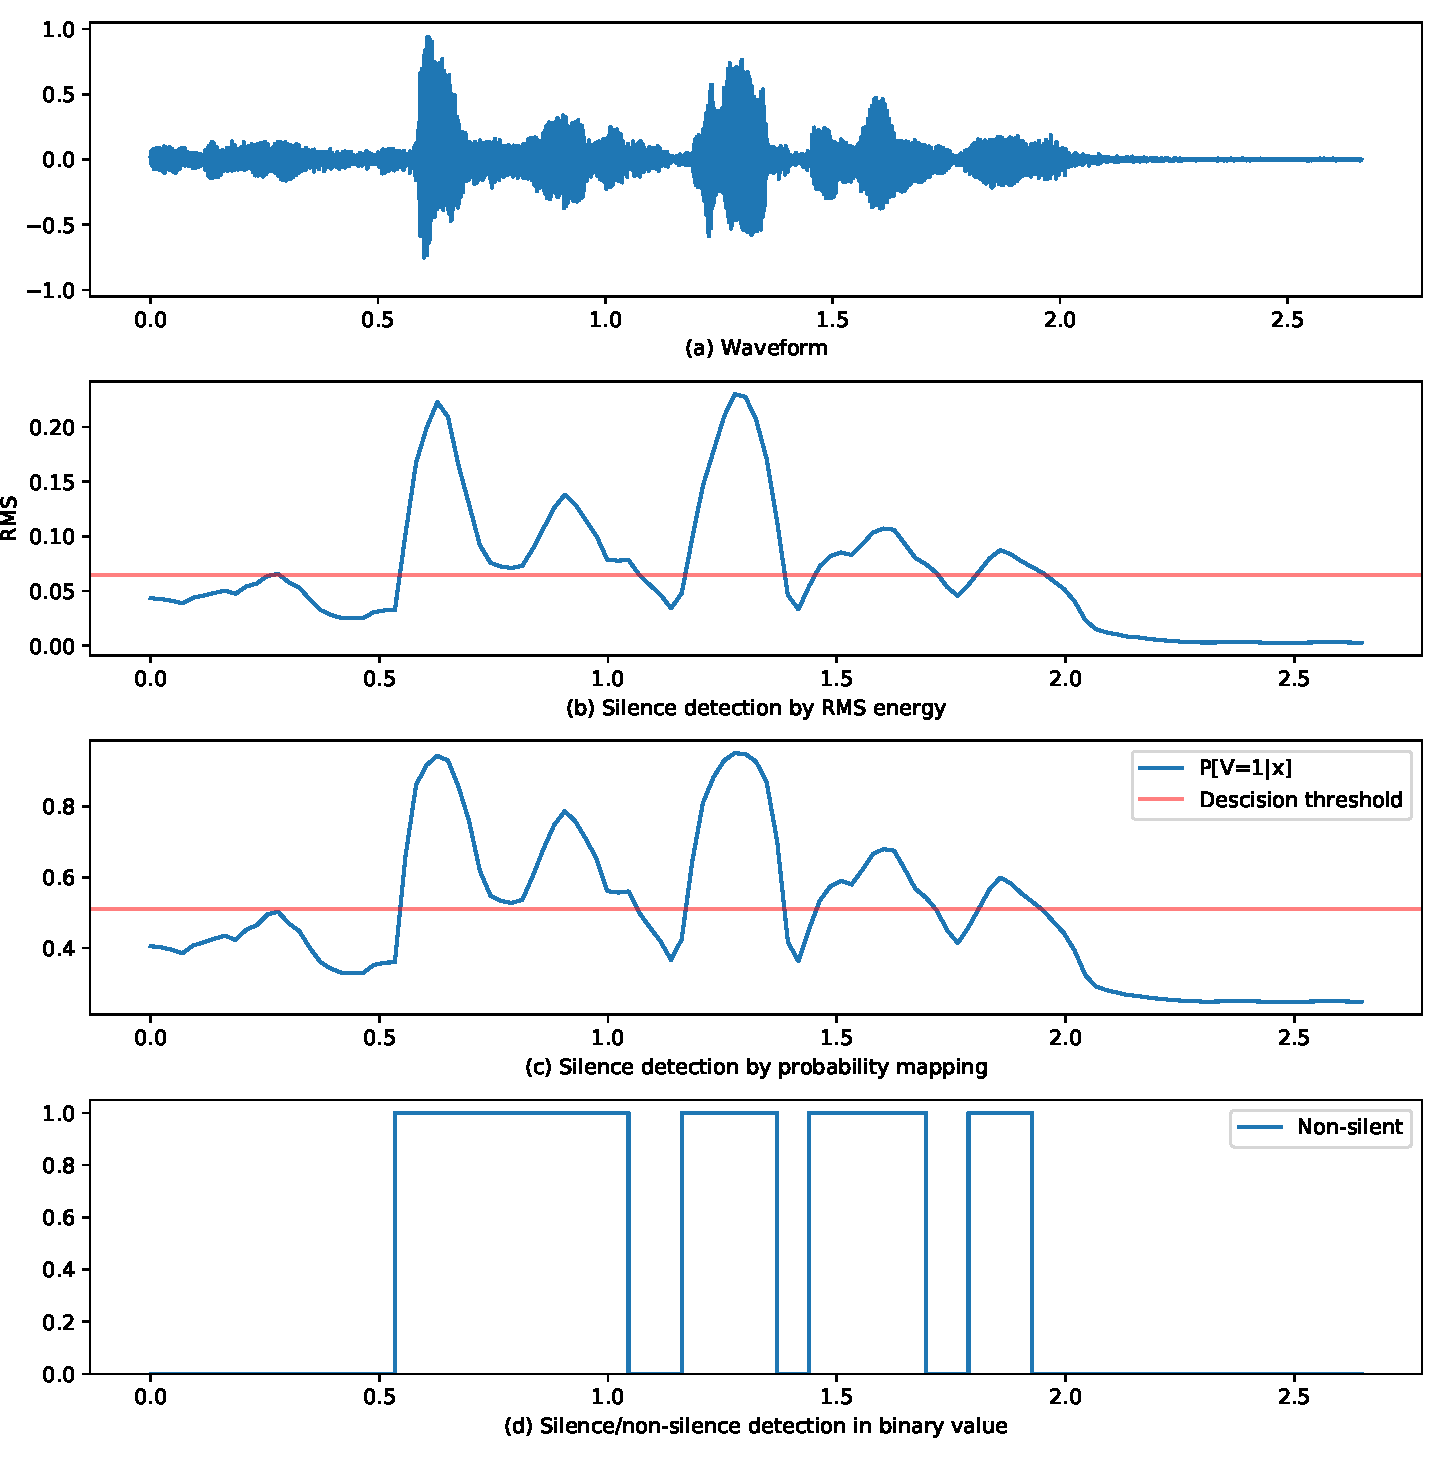
\includegraphics[width=\textwidth]{../fig/silence.pdf}
  \caption{Calculation of silence region in speech}
  \label{fig:silence}
\end{figure}

In practice, using threshold $\tau$ as percentage from maximum values is more
intuitive while it gives the similar result. Additionally, (minimum) duration of
silence is another important parameter. The minimum number of samples to be
removed represents duration of pause in speech communication, which has been
studied thoroughly \cite{Campione2002}. These two parameters, silence $\tau$
and duration $d$ can be used to experiment with for removing silence region and 
extract the acoustic features from these regions.

Three different thresholds and durations were performed to remove silence from
speech dataset. For the threshold, the value of 0.01\%, 0.1\%, and 5\% were
examined while for durations were 10 ms 60 ms and 100 ms. The results are shown
in Table \ref{tab:sil_remove}. As baseline method, MLP with Mean+Std of
pyAudioAnalysis features (without deltas, 68 dimension) were used. The baseline
method gains 0.458 of average CCC score. Among nine combinations of duration and
threshold for removing silences where acoustic features were extracted, only
one result shows a higher performance than the baseline. This result in line
with previous research (\cite{Atmaja2019, Tian2015a, Aguilar2020,Fayek2017}), in
which special adjustments are needed to take the benefit of threating silence
pause region in speech.

\begin{table}
  \caption{Result of using different duration and threshold factor for
  removing silence on dimensional SER performance}
  \begin{center}
  \begin{tabular}{c | c | c c c c}
    \hline
    duration (ms)   & threshold (\%) &  V & A & D & Mean \\
    \hline \hline
    10	& 0.1	& 0.283	& 0.640	& 0.454	& 0.459 \\
    60	& 0.1	& 0.279	& 0.625	& 0.453	& 0.452 \\
    100	& 0.1	& 0.281	& 0.629	& 0.456	& 0.455 \\
    10	& 1	& 0.234	& 0.560	& 0.418	& 0.404 \\
    60	& 1	& 0.255	& 0.574	& 0.425	& 0.418 \\
    100	& 1	& 0.276	& 0.571	& 0.429	& 0.425 \\
    10	& 5	& 0.205	& 0.568	& 0.393	& 0.389 \\
    60	& 5	& 0.209	& 0.567	& 0.398	& 0.391 \\
    100	& 5	& 0.205	& 0.557	& 0.393	& 0.385 \\
    \hline
  \end{tabular}
  \label{tab:sil_remove}
  \end{center}
\end{table}

\subsection{Dimensional SER with silence pause features}
% other research that say silence is useful for emotion
Tian et al. \cite{Tian2015a} argued that silence is an effective cue for
recognizing emotion.  Using this idea, Fayek et al. used silence as an
additional category for detecting emotion categories from speech signal. Silent
pause length also plays an important role in ascribing emotions based on
psychoacoustics experiment \cite{Tisljar-Szabo2014}. These assumptions along
with their results are motivation to use silence as a feature for dimensional
SER.

There are several ways to count silence pause features in speech. A
straightforward way is by detecting the number of silence regions and compared
to it to whole utterance. The result is a portion of silence region over
speech. Although this method may represent silent pause more precisely, there
are more effort needed to align timing of spoken words and silence region
manually to obtain more accurate result. Alternatively, silent pause detection
can be done on frame basis calculation with fixed length samples (of speech
signals). A frame, then, can be categorized as silence or non silence by a
specific rule.

A silent pause feature, in this research, is defined as the proportion of
silent frames among all frames in an utterance. In human communication, the
proportion of silence in speaking depends on the speaker's emotion. For
example, a happy speaker may have fewer silences (or pauses) than a sad
speaker. The proportion of silence in an utterance can be calculated as

\begin{equation}
  \label{eq:sil_ratio}
  S = \frac{N_{s}}{N_{t}},
\end{equation}
where $N_s$ is the number of frames categorized as silence (silent frames), and
$N_t$ is the total number of frames. A frame is categorized as silent if it does
not exceed a threshold value defined by multiplying a factor by a root mean
square (RMS) energy, $X_{rms}$. Mathematically, this is formulated as

\begin{equation}
 th = \alpha \times \overline{X_{rms}},
\end{equation}

This silence feature is similar to the disfluency feature proposed in
\cite{moore2014word}. In that paper, the author divided the total duration of
disfluency by the total utterance length for $n$ words. Figure
\ref{fig:silence_fig} illustrates the calculation of our silence feature. If
$X_{rms}$ from a frame is below $th$, then it is categorized as silent, and the
calculation of equation \ref{eq:sil_ratio} is applied.

Two important parameters for this silent pause features then can be
investigated,
\begin{enumerate}
  \item threshold factor ($\alpha$), and
  \item silent pause duration.
\end{enumerate}
Both parameters are investigated in this study. A factor of 0.1, 0.2, and 0.3 
from averaged RMS values are evaluated for silence threshold factors.
Silent pause duration of 200 ms, 500 ms, and 1 s are also investigated based 
on the study of the division of pause \cite{Campione2002}.

\begin{figure}[htbp]
  \centering
  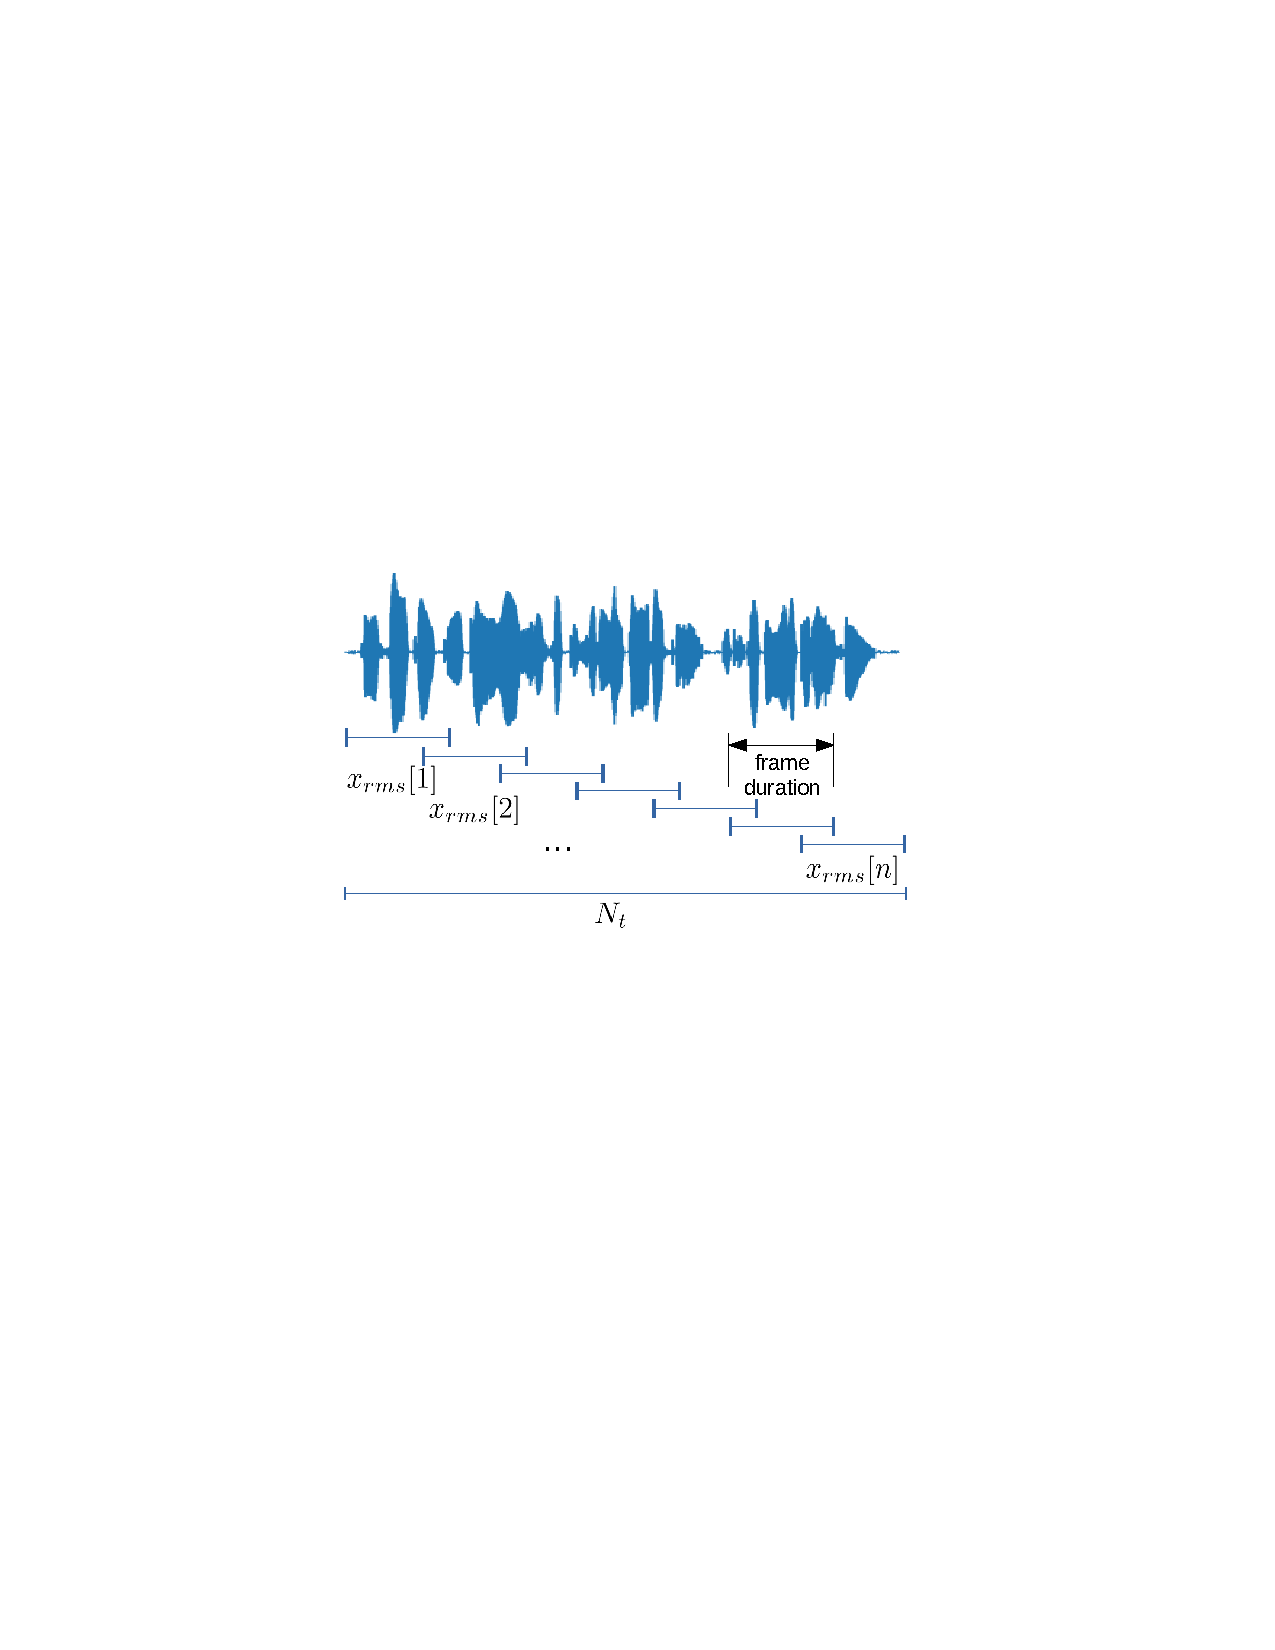
\includegraphics[width=0.8\textwidth]{../fig/silence_fig.pdf}
  \caption{Silent pause features calculation}
  \label{fig:silence_fig}
\end{figure}

Figure \ref{fig:msp_threshold} shows the use of different threshold factors 
in determining silent pause features. Clearly, it shows that the lower 
threshold factor, the smaller number of silence frames correspond to 
silent pause features. Thus, the choice of silence threshold factor 
is also a critical aspect when calculating silent pause features 
apart from the silent pause duration.

\begin{figure}[htbp]
  \centering
  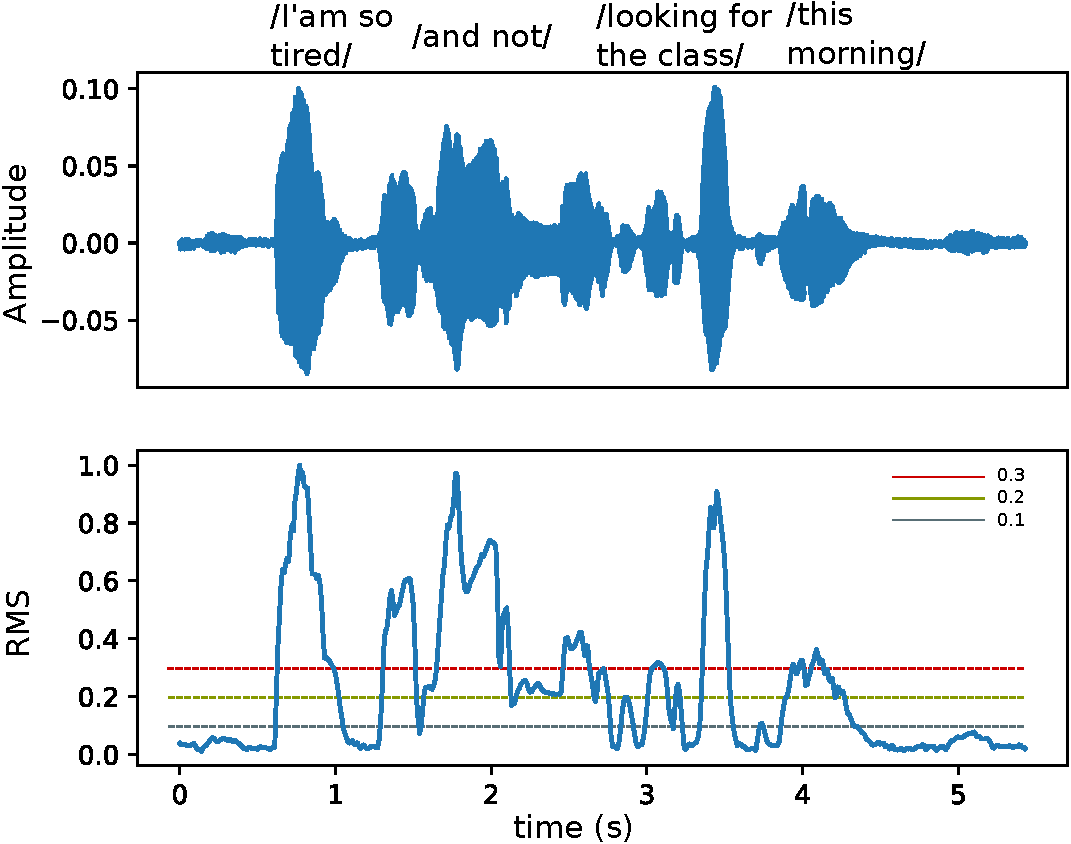
\includegraphics[width=0.8\textwidth]{../fig/msp_sa01a-crop}
  \caption{Different silent threshold factors on normalized RMS}
  \label{fig:msp_threshold}
\end{figure}

\section{Acoustic features aggregation}
The final issue to discuss in this chapter is to choose which aggregation
method works best for dimensional SER from acoustic features. It is common in
processing audio to split an utterance (or story) into chunks. The goal is for
fast processing as well as for reducing the size of recorded/analyzed audio
data. While the label is only given per utterance, acoustic features extraction
is performed on chunk-based processing, either using LLDs or HSFs. Thus, two
options exist: whether aggregating input features to have single label per
utterance or aggregating outputs with many labels for a single utterance. For
the latter method, the label to represent a single story from many chunk labels
can be performed by a such method, e.g., majority voting.  

% telling acoustic features used
Seven types of LLDs from LibROSA features extractor \cite{McFee2020} extracted
for acoustic input features: MFCCs (40 coefficients), chroma (12),
mel-spectrogram (128), spectral contrast (7), tonal centroid (6), deltas of
MFCCs (40), and deltas-deltas of MFCCs (40).  This feature set is adopted from
\cite{Atmaja2020c}. In total, there are 273 features on each frame. Following
the previous success in using global features for determining region of
analysis, Mean+Std from these 273 LLDs were extracted resulting 546-dimensional
functional features.

% feature aggregation, % why mean and max
Input features aggregation is a method to choose which features to represent a
set of data (story) given many recordings (chunks). Statistical functions were
widely used to aggregate many measurements. The choice of mean and maximum
values for acoustic feature aggregation is based on assumption that acoustic
features representing emotion either from mean values (e.g., mean intonation)
or maximum values (e.g., high pitch in specific speech region when expressing
fear or happy). In maximum aggregation, the highest column vector value of
acoustic features (Mean+Std from LLDs) for each chunk on the same stories. By
using these methods, each story has the same $n$-dimensional feature
vector depend on extracted acoustic features. The similar approach was
conducted for mean values feature aggregation. Figure
\ref{fig:input_aggregation} shows acoustic input aggregation from chunks to
story. 

\begin{figure}[htbp]
  \centering
  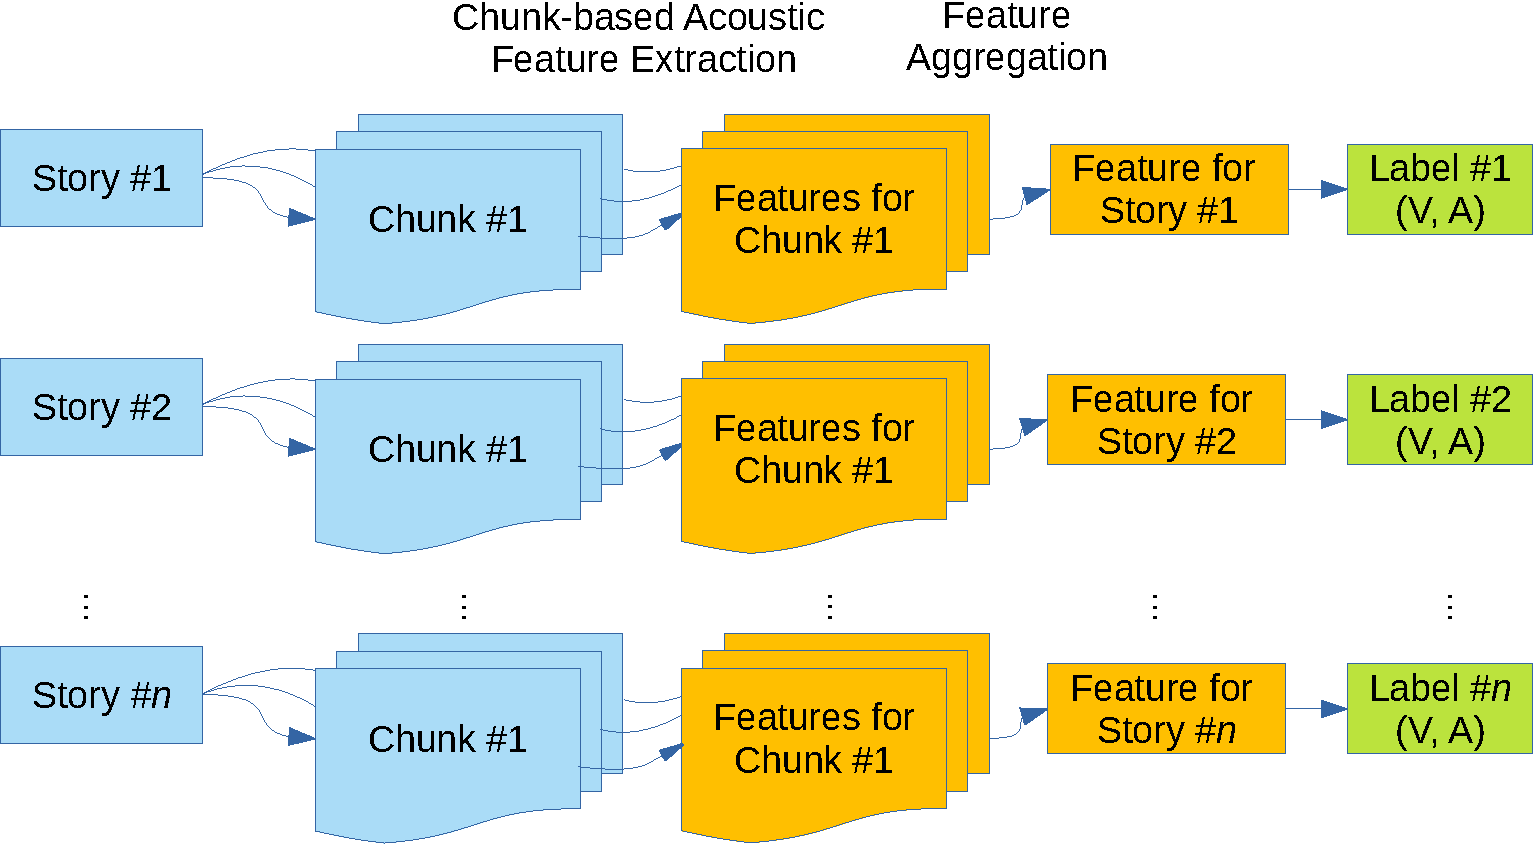
\includegraphics[width=.7\textwidth]{../fig/feature_aggregation-crop.pdf}
  \caption{Flow diagram of acoustic input features aggregation}
  \label{fig:input_aggregation}
\end{figure}

% majority voting
Output aggregation is often performed by majority voting. The use of majority
voting in SER has been implemented in various technique \cite{Sezgin2012,
Elbarougy2019}. Majority voting method were often used to choose the final
label over different classifiers (known as \textit{ensemble} method). However,
the majority voting defined in this study closer its original term; the most
frequent classes is chosen among them to represent the data. In the INTERSPEECH
2020 elderly sub-challenge (ESC), the dataset provided audio files as chunks,
parts of an utterance/story. Acoustic features (frame-based processing and
statistical functions) were extracted per this chunk and forwarded to a
classifier. Thus, in a single story, there are many labels with regard to the
number of chunks. Majority voting choose the most frequent labels to represent
a story (Figure \ref{fig:output_aggregation}).

\begin{figure}[htbp]
  \centering
  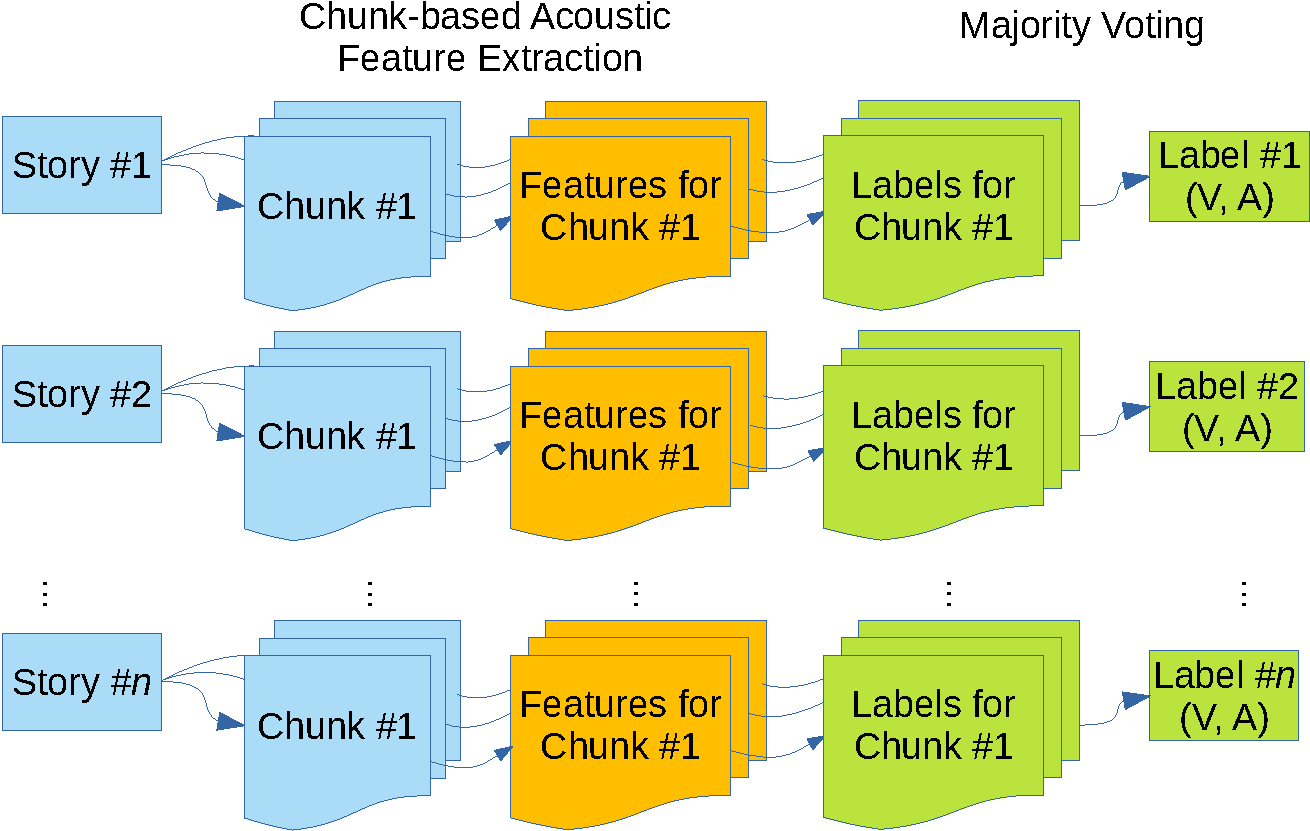
\includegraphics[width=.7\textwidth]{../fig/majority_voting-crop.pdf}
  \caption{Flow diagram of acoustic outputs aggregation (majority voting)}
  \label{fig:output_aggregation}
\end{figure}



% result
In comparing mean vs. maximum aggregation methods, it is found that mean
aggregation lead to higher UAR score than maximum aggregation in development
partition. All results from mean input aggregation attain higher score than
baseline majority voting. Table \ref{fig:input_aggregation} also shows
that mean input aggregation works better than mean output aggregation. This
finding suggests that using all chunks (by averaging) is better than choosing
one value from a chunk (by maximum value). This evidence also supports the
previous global features approach as solution to choose region of analysis of
acoustic features.


% Mean+Std from Compare dataset
\begin{table}
  \caption{UAR results on development set: Unimodal acoustic features aggregation
  vs. baseline \cite{Schuller} (Interspeech 2020 ComParE Elderly
  Emotion Sub-Challenge dataset)}
    \label{tab:acoustic_aggregation}
    \begin{center}
    \begin{tabular}{l c c c c c c}
    \hline 
Features  & \multicolumn{2}{c}{Majority Voting \cite{Schuller} } &
\multicolumn{2}{c}{Mean Input Agg.}      & \multicolumn{2}{c}{Max Input Agg.} \\
              & V & A & V & A & V & A \\   
      \hline \hline
      LibROSA Mean+Std  & - & - & \textbf{45.1}  & 38.3  & 42.7 & 39.7 \\
      ComParE & 33.3  &   39.1  & 43.4  & 42.7  & \textbf{45.3} & 37.0 \\
      BoAW-125  & 38.9  &   42.0& 44.6 & \textbf{45.7} & 44.6  & 40.1 \\
      BoAW-250  & 33.3  & 40.5  & 43.0  & 40.8  & 39.6  & 37.6 \\
      BoAW-500  & 38.9  & 41.0  & 42.6  & 41.0  & 42.9  & 37.9 \\
      BoAW-1000 & 38.7  & 30.5  & 43.5  & 41.5  & 40.2  & 39.8 \\
      BoAW-2000 & \textbf{40.6}  & 39.7  & 41.9  & 44.8  & 43.4  & 40.1 \\
      ResNet50  & 31.6  & 35.0  & 36.5  & 36.7  & 37.1  & 39.0 \\
      AuDeep-30 & 35.4  & 36.2  & 38.4  & 42.1  & 42.8  & 35.6 \\
      AuDeep-45 & 36.7  & 34.9  & 39.5  & 40.5  & 39.3  & 33.3 \\
      AuDeep-60 & 35.1  & \textbf{41.6}  & 43.4  & 42.1  & 40.7  & 41.4 \\
      AuDeep-75 & 32.7  & 40.4  & 41.9  & 44.4  & 40.9  & \textbf{43.3} \\
      AuDeep-fused  & 29.2  & 36.3  & 43.6  & 39.5  & 42.2  & 39.3 \\
    \hline
    \end{tabular}
  \end{center}
  \end{table}

% why not use features from all chunks, i.e., whithout any aggregation method
The use of aggregation methods reduces feature dimension (for input to
classifier) and computational complexity. Using all chunks to process the data,
e.g., without feature aggregation increase computation load, increases
computational complexity. The number of samples became larger according to the
number of chunks. However, the UAR score is low. Using feature aggregation not
only reduces complexity and feature dimension, but also increase the
performance score.

% The content following two sections can be included in summary and previous
% sections
% \section{Effect of Different Acoustic Features}
% \section{Effect of Different Classifiers}
\section{Summary}
This chapter 
\begin{table}
  \caption{Summary of study on dimensional SER using acoustic features}
  \begin{center}
  \begin{tabular}{l| ccc}
  \hline
  Issue & \multicolumn{3}{c} {Proposed method} \\
  \hline \hline
  Region of analysis  & \mybox{frames} & & utterance (fixed length) \\
  Silence region   & \mybox{removing silence}  & \mybox{keeping silence} &
  utilizing silence\\
  Aggregation method  & input aggregation & & \mybox{output aggregation} \\
  \hline
  \end{tabular}
\end{center}
\end{table}
